%!BIB program=biber

\documentclass[12pt,aspectratio=169]{beamer} %类型为文章
\usepackage[UTF8]{ctex} %中文编码宏
\usepackage{multicol} %分栏控制宏
\usepackage{hyperref} %超链接宏
\usepackage{lastpage} %总计页的宏
\usepackage{color} %颜色控制宏
\usepackage{graphicx} %图片插入宏
\usepackage{subfigure} %子图插入宏
\usepackage{animate} %动画插入宏
\usepackage{multirow} %纵向合并宏
\usepackage{makecell} %表格换行宏
\usepackage{amsmath} %公式插入宏
\usepackage{unicode-math} %公式样式宏
\usepackage{gbt7714} %国标引用宏
\usepackage{url} %网页链接宏
\usepackage{doi} %doi号宏
\usepackage{svg}
\renewcommand{\vec}[1]{\boldsymbol{#1}} %设置向量样式

\usetheme{Berlin}
\usecolortheme{beaver}

\linespread{1.2} %行距
\setlength{\parskip}{0.5em} %段落间距
\setlength{\parindent}{2em} %缩进距离

\setmathfont{Cambria Math} %设置数学公式样式
%\bibliographystyle{gbt7714-numerical} %设置参考文献样式

%\logo{
\includegraphics[height=0.1\textwidth]{images/SCU_logo.pdf}}
%\setbeamertemplate{background}{
\includegraphics[height=\paperheight]{images/SCU_logo.pdf}}
\setbeamertemplate{itemize items}{$\blacksquare $}
\setbeamertemplate{caption}[numbered]


\title{工作进展回报} %设置标题
\subtitle{对傅里叶重建算法的理解}
\author{Julian OU} %设置作者
\institute[SCU]{\textit{College of Physics, Sichuan University, Chengdu 610064, China}}
\date{\today} %设置日期

\begin{document}
\maketitle %插入标题

\AtBeginSection{
    \begin{frame}
        \frametitle{目录}
        \tableofcontents[currentsection,subsectionstyle=hide]
    \end{frame}
}

\AtBeginSubsection{
    \begin{frame}
        \subsectionpage
    \end{frame}
}

\section{前人工作(ER、HIO、OSS)}

\begin{frame}
    \frametitle{基本构想}
    \begin{figure}
        \subfigure{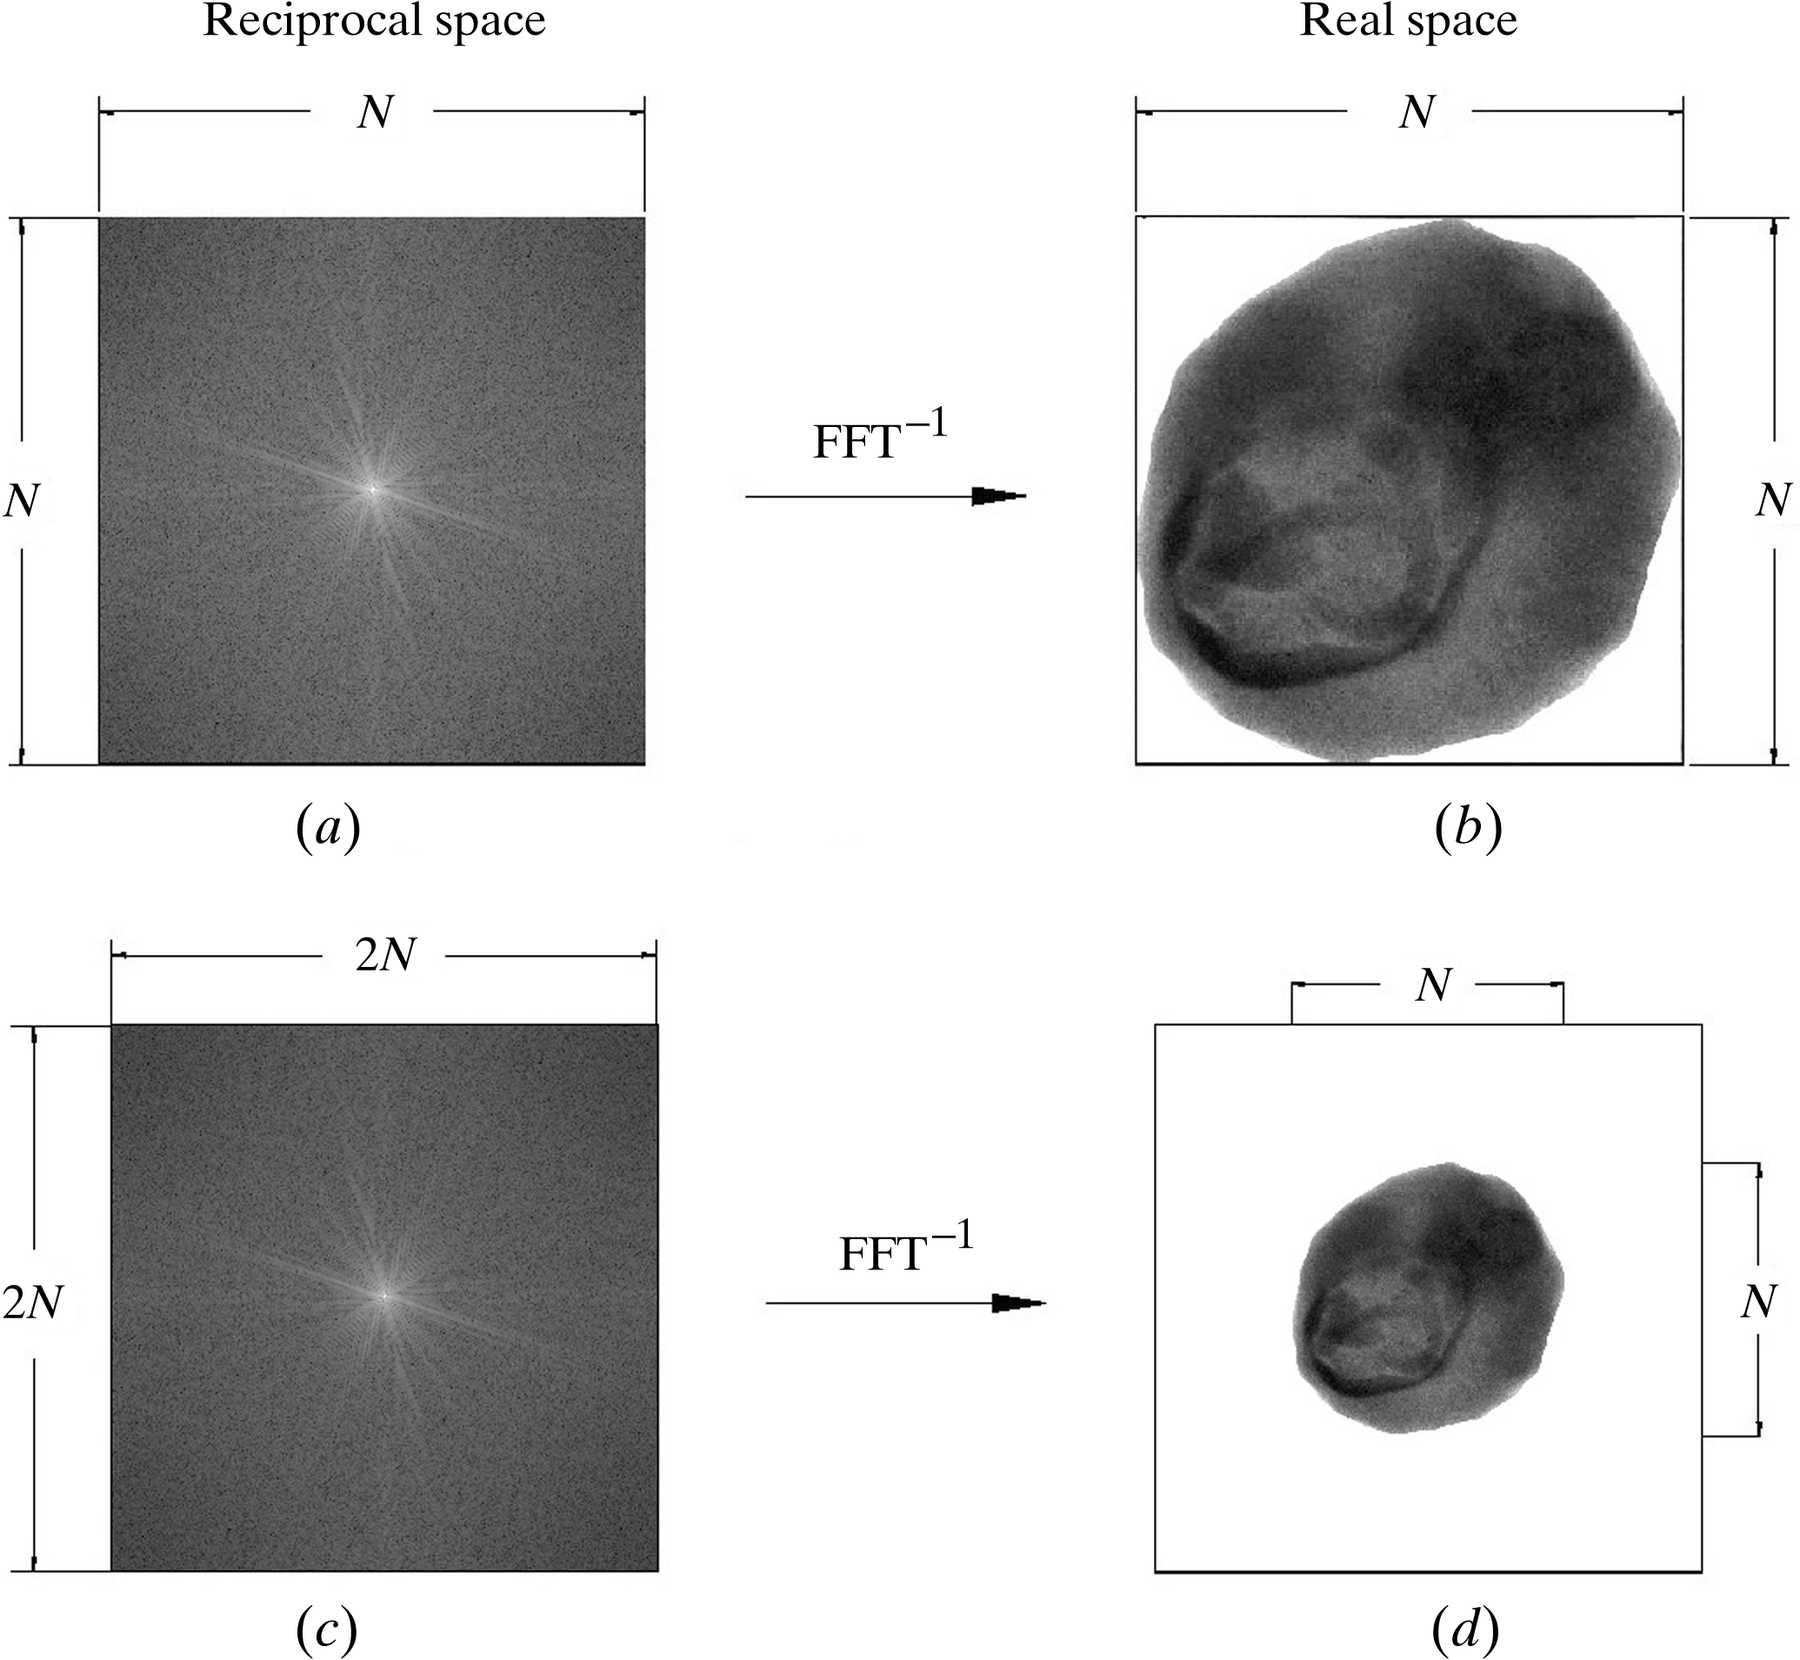
\includegraphics[height=5cm]{images/bk0084fig1mag.jpg}}
        \qquad
        \subfigure{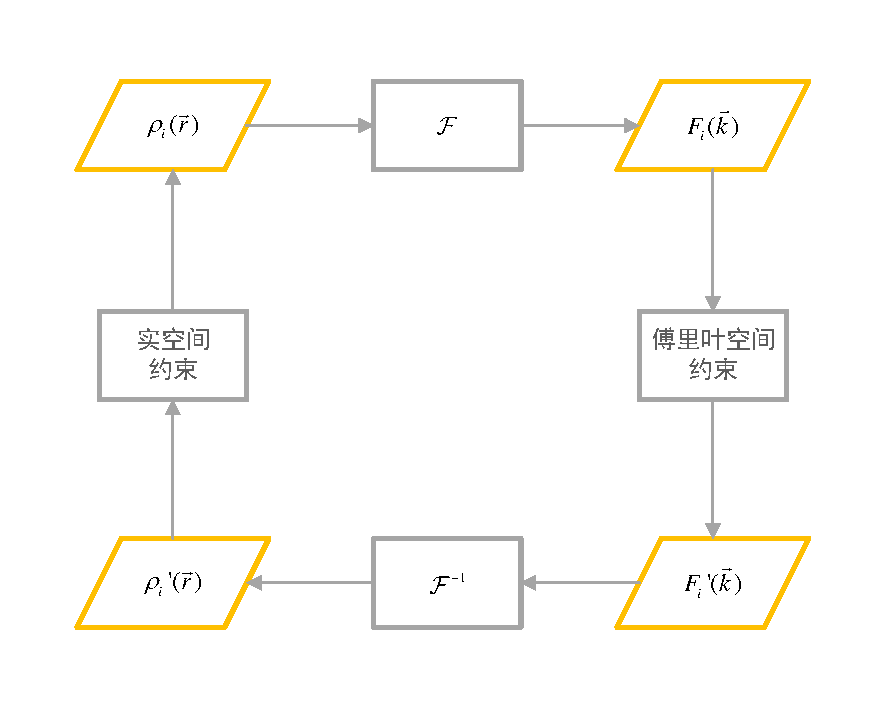
\includegraphics[height=5cm]{images/1.pdf}}
    \end{figure}1
\end{frame}

\begin{frame}
    \frametitle{ER-HIO}
    \begin{figure}
        \subfigure{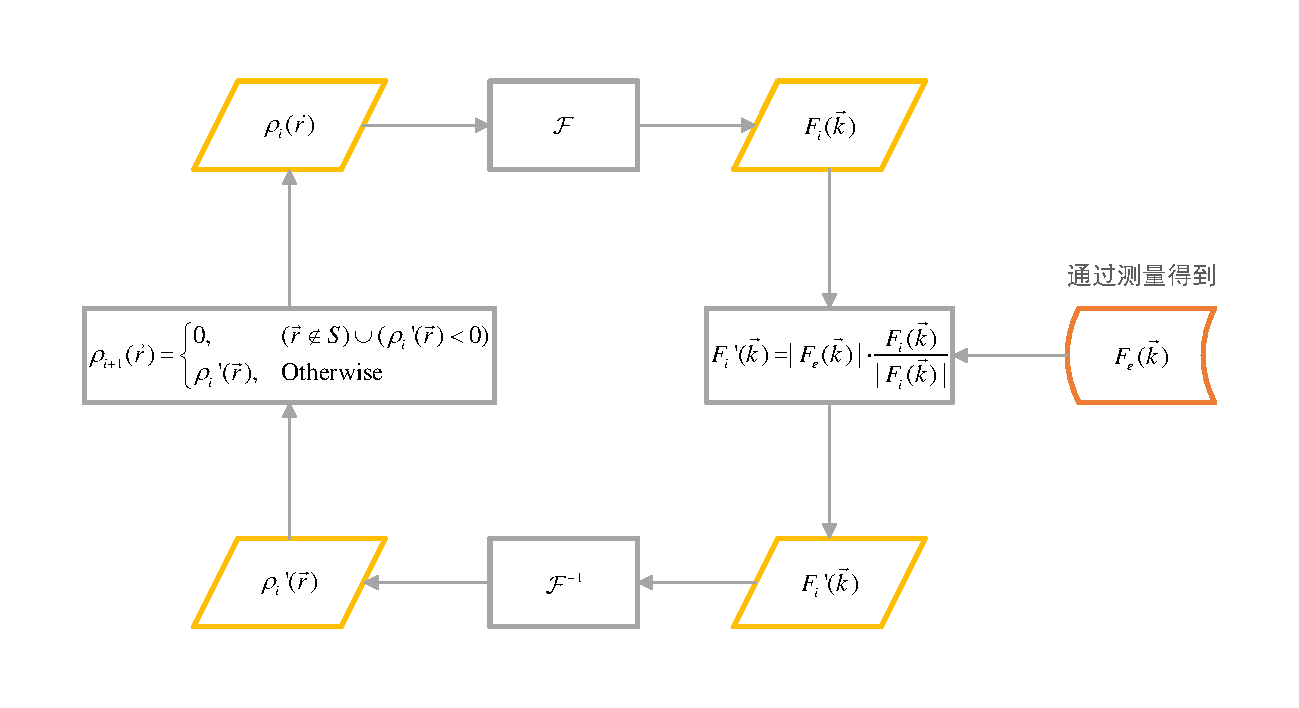
\includegraphics[height=3.6cm]{images/2.pdf}}
        \subfigure{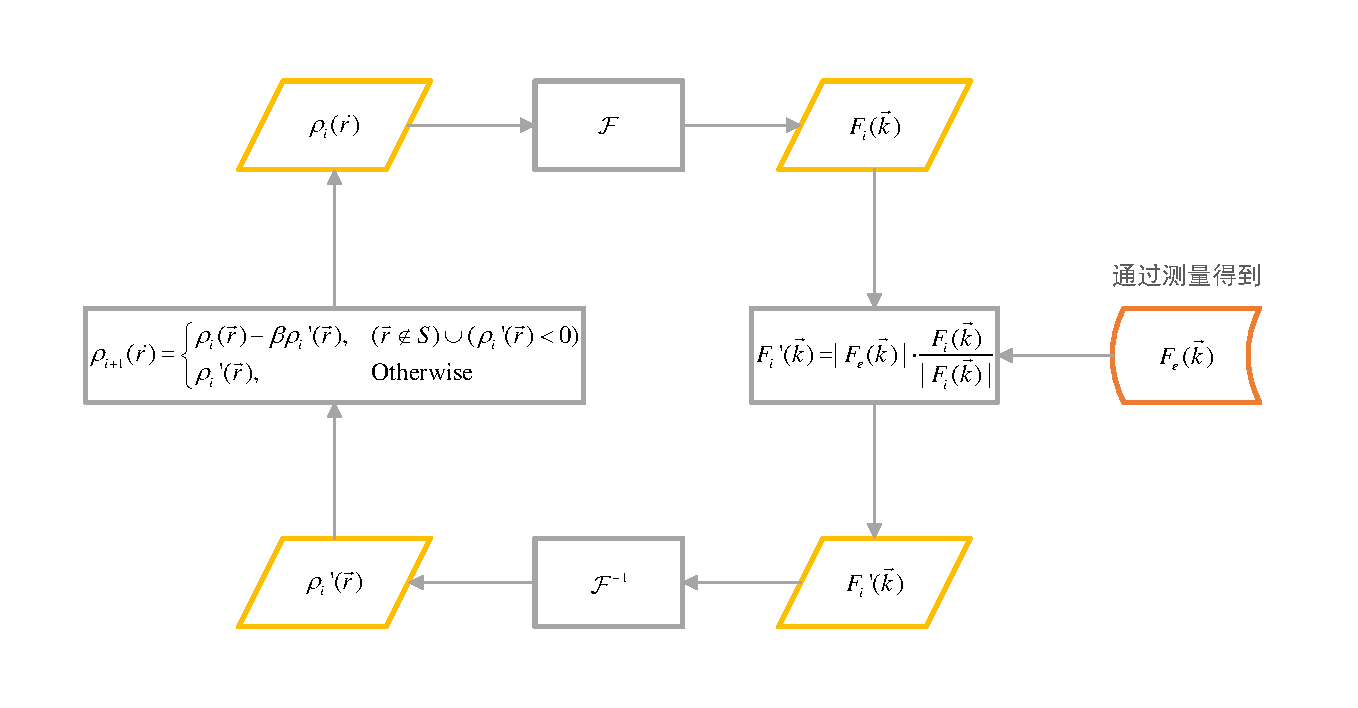
\includegraphics[height=3.6cm]{images/3.pdf}}
    \end{figure}
\end{frame}

\begin{frame}
    \frametitle{OSS}
    \begin{figure}
        \subfigure{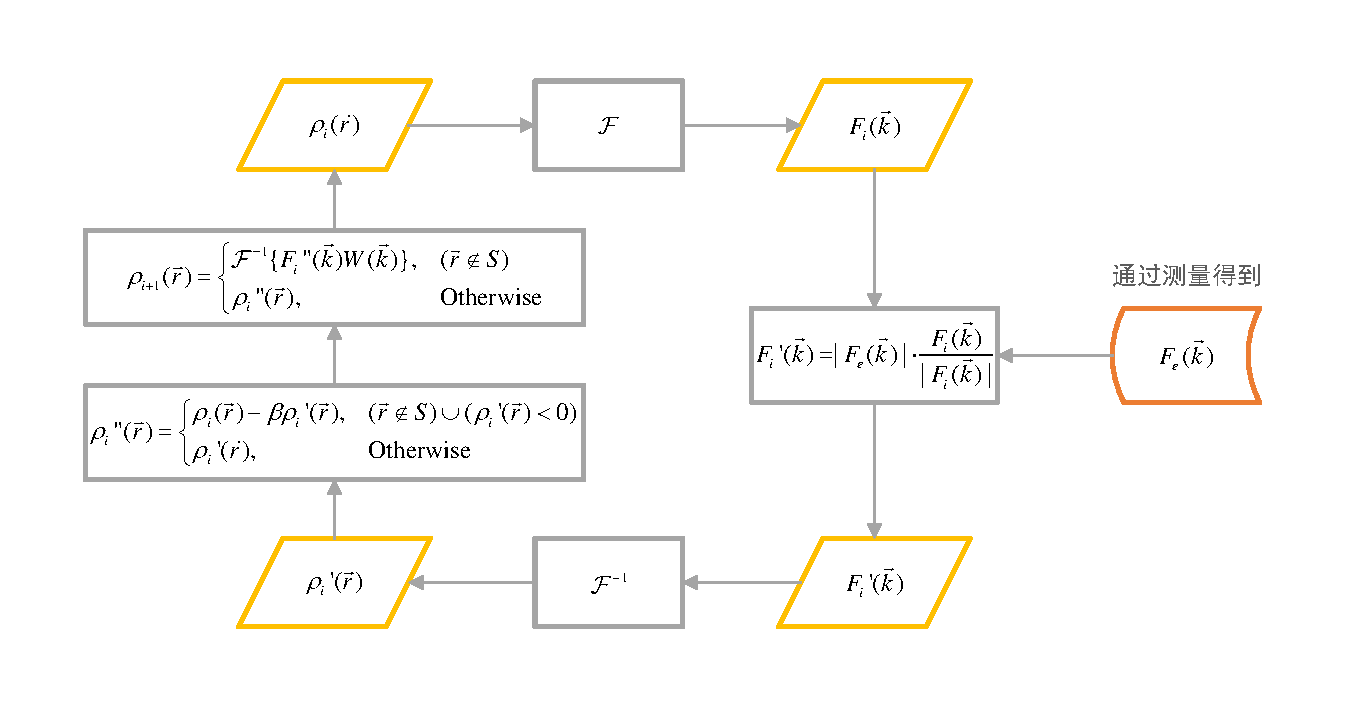
\includegraphics[height=5cm]{images/5.pdf}}
        \subfigure{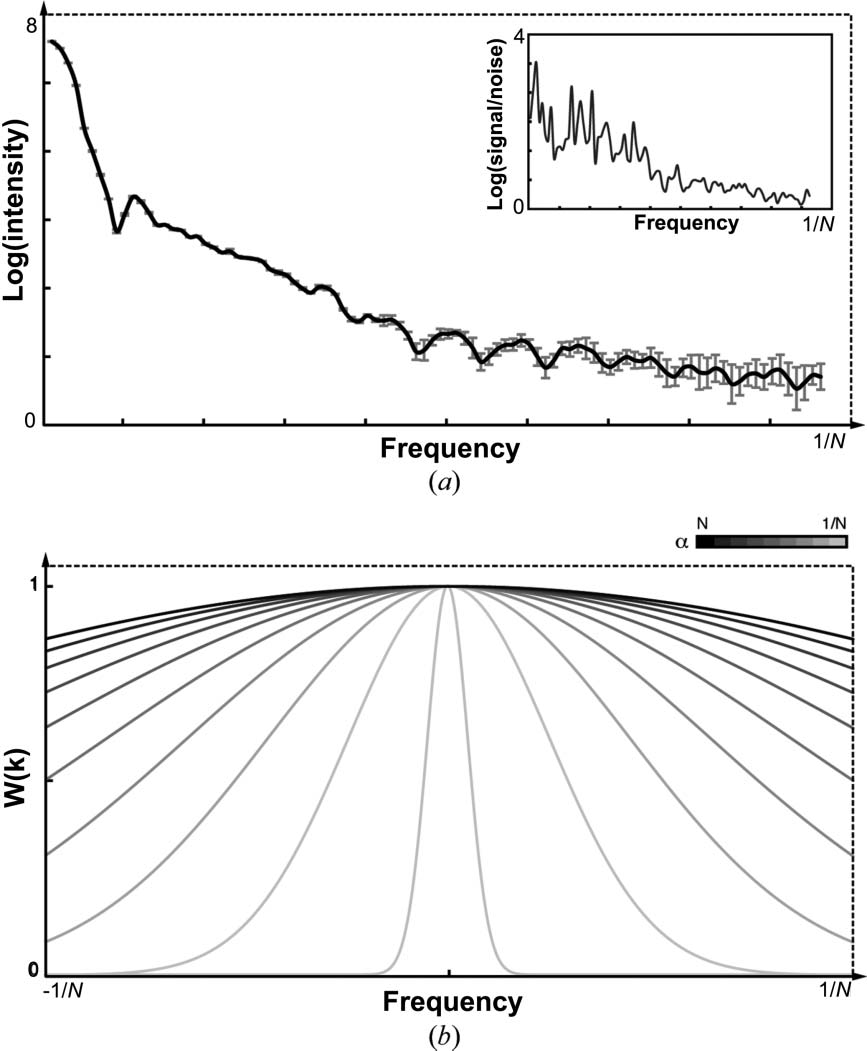
\includegraphics[height=5cm]{images/OSS_JAC_2013Oversampling smoothness-an effective algorithm.jpg}}
    \end{figure}
\end{frame}

\section{算法改进(Frequency Split, FS)}

\subsection{结果}

\begin{frame}
    \frametitle{重建用图}
    \begin{columns}
        \begin{column}{0.7\textwidth}
            \begin{figure}
                \subfigure[Lenna原图]{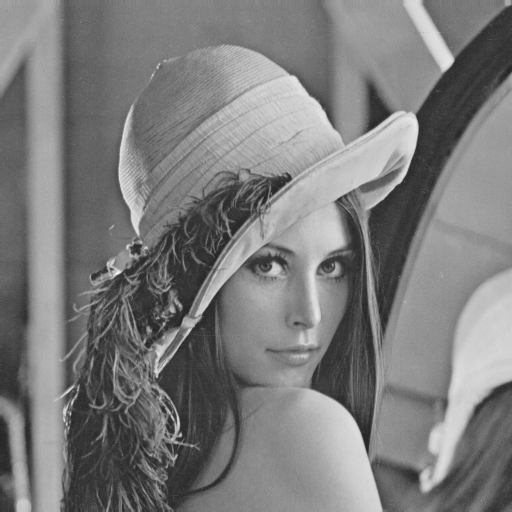
\includegraphics[height=4cm]{images/Lenna_gray_180d.png}}
                \qquad
                \subfigure[Lenna衍射图案]{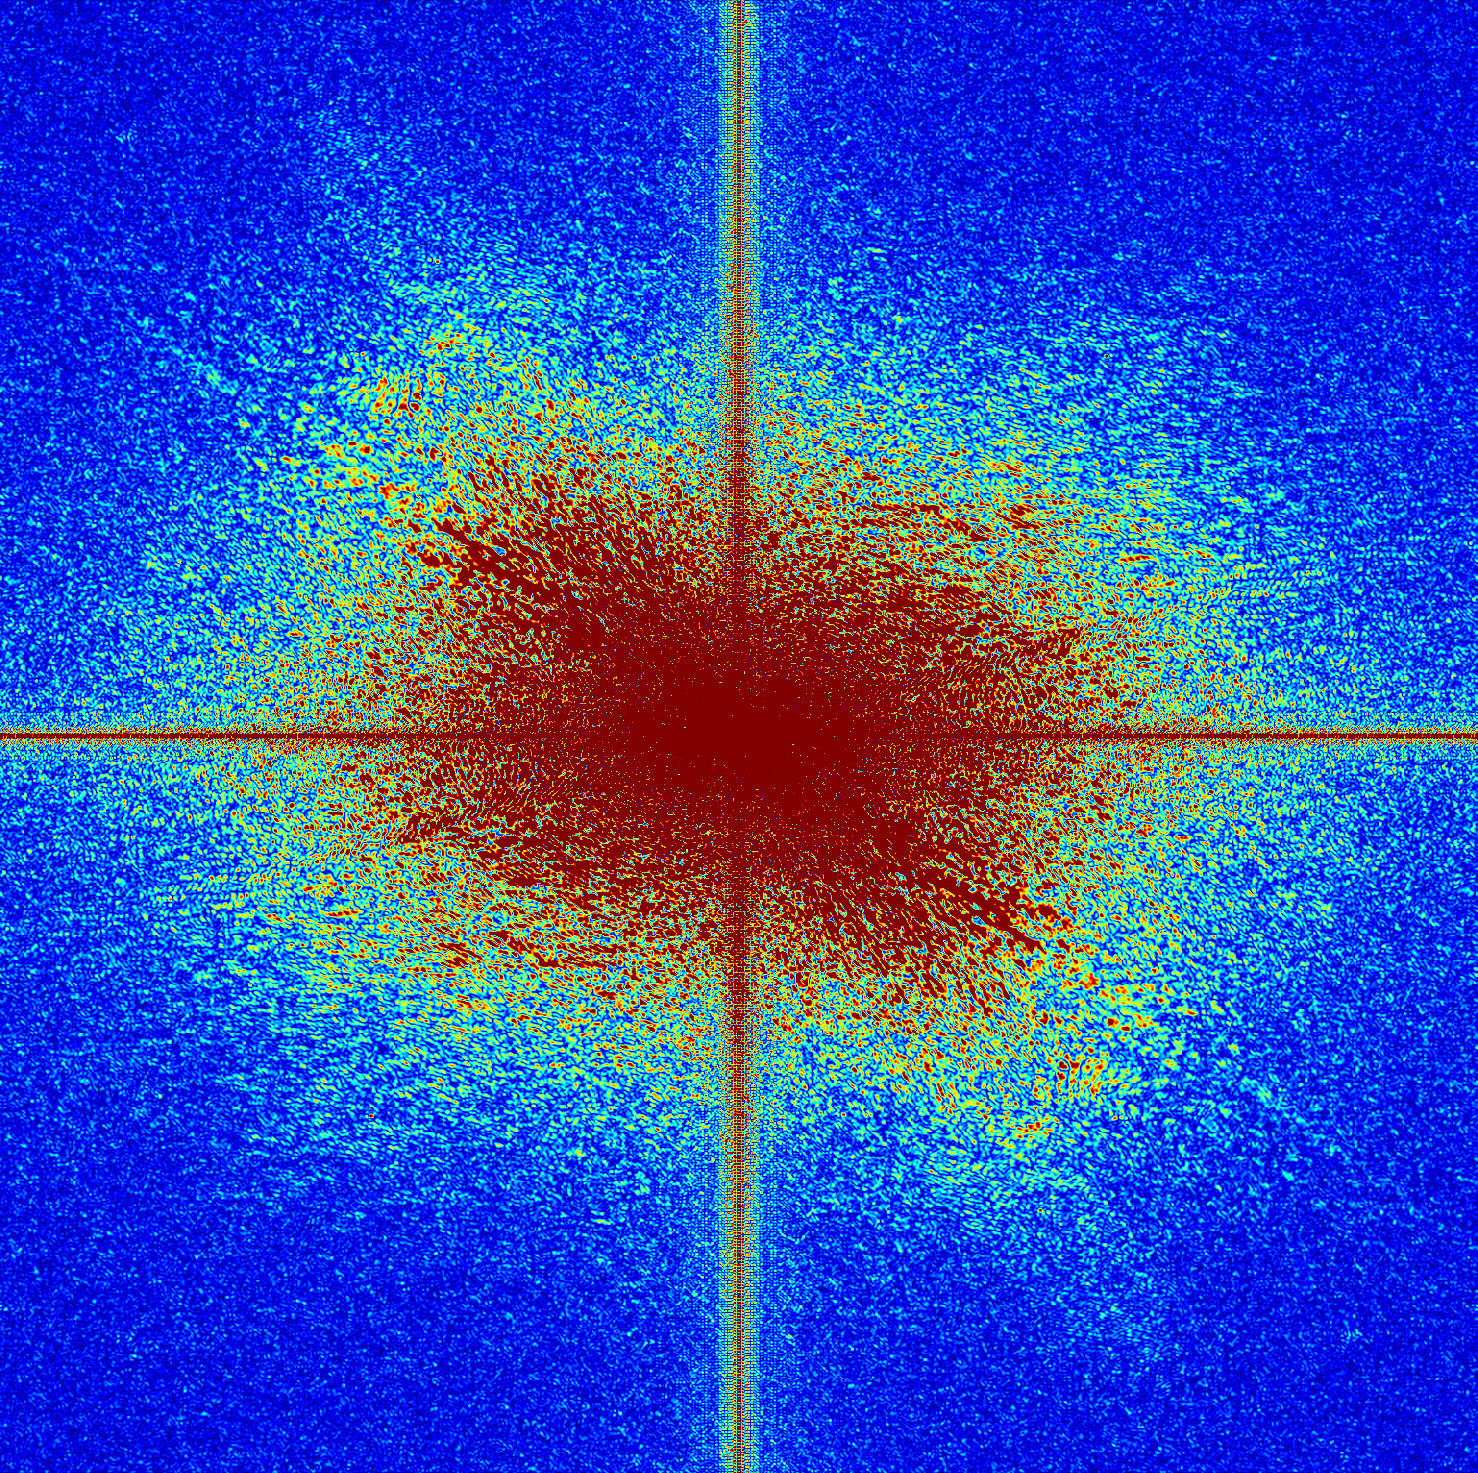
\includegraphics[height=4cm]{images/Lenna_fourier.png}}
            \end{figure}
        \end{column}
        \begin{column}{0.3\textwidth}
            \begin{block}{模拟衍射}
                (g)为Lenna的512$\times$512原始图像;

                (h)为过采样率为3的模拟衍射图像。
            \end{block}
        \end{column}
    \end{columns}
\end{frame}

\begin{frame}
    \frametitle{重建结果}
    \begin{columns}
        \begin{column}{0.7\textwidth}
            \begin{figure}
                \subfigure[ER-HIO重建图]{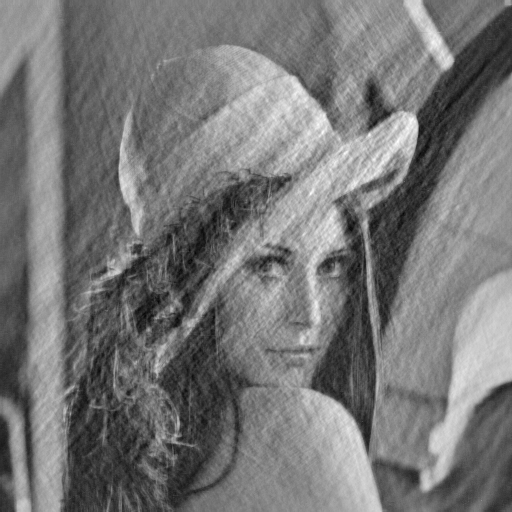
\includegraphics[height=4cm]{images/Lenna_test_1000_180d.png}}
                \qquad
                \subfigure[ER-HIO-FS重建图]{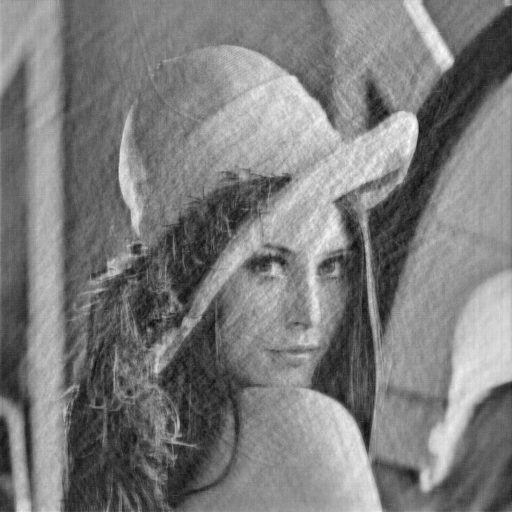
\includegraphics[height=4cm]{images/Lenna_test_RL_0.5_re_0.5.png}}
            \end{figure}
        \end{column}
        \begin{column}{0.3\textwidth}
            \begin{block}{重建方法}
                (i)2000(20HIO+5ER);
                
                (j)使用线性函数滤波,分别对高频和低频部分用ER-HIO分别重建1000(20HIO+5ER),再叠加的图像。
            \end{block}
        \end{column}
    \end{columns}
\end{frame}

\begin{frame}
    \frametitle{误差分析}
    \begin{columns}
        \begin{column}{0.7\textwidth}
            \begin{figure}
                \subfigure[ER-HIO误差图]{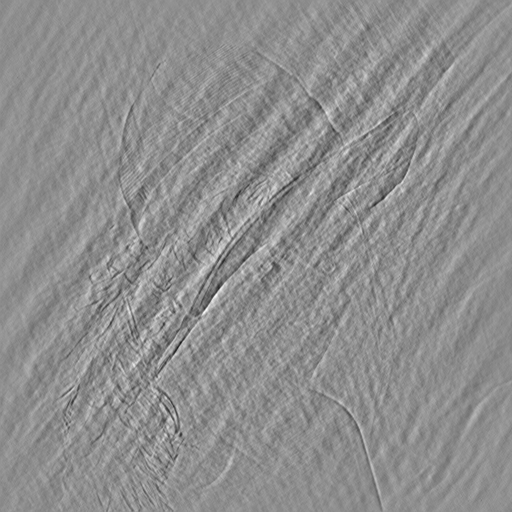
\includegraphics[height=4cm]{images/rms_1000.png}}
                \qquad
                \subfigure[ER-HIO-FS误差图]{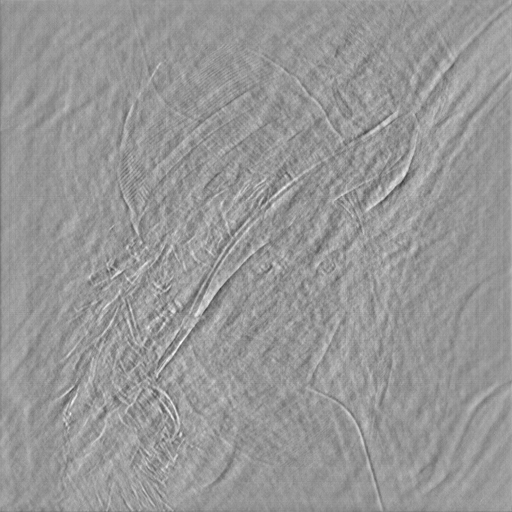
\includegraphics[height=4cm]{images/rms_0.5_re.png}}
            \end{figure}
        \end{column}
        \begin{column}{0.3\textwidth}
            \begin{block}{均方误差}
                \small \begin{align*}
                    &E_{rms}=\sqrt{\frac{\sum_i^n (X_{obs}-X_{ori})^2}{n}}\\
                    &E_{ER-HIO}=14.0177\\
                    &E_{ER-HIO-FC}=11.0223
                \end{align*}
            \end{block}
        \end{column}
    \end{columns}
\end{frame}

\subsection{方法}

\begin{frame}
    \frametitle{应用滤波器}
        \begin{columns}
            \begin{column}{0.5\textwidth}
                \begin{figure}
                    \includesvg[height=5cm]{images/0.5-1.svg}
                \end{figure} 
            \end{column}
            \begin{column}{0.4\textwidth}
                \begin{block}{分波段}
                    此处应用线性函数进行滤波,经过测试,如图所示的线性函数滤波后重建效果最佳。

                    将来还会考虑使用其他非线性滤波器进行滤波。
                \end{block}
            \end{column}
        \end{columns}
\end{frame}

\begin{frame}
    \frametitle{衍射图案对比}
        \begin{figure}
            \subfigure[滤波前]{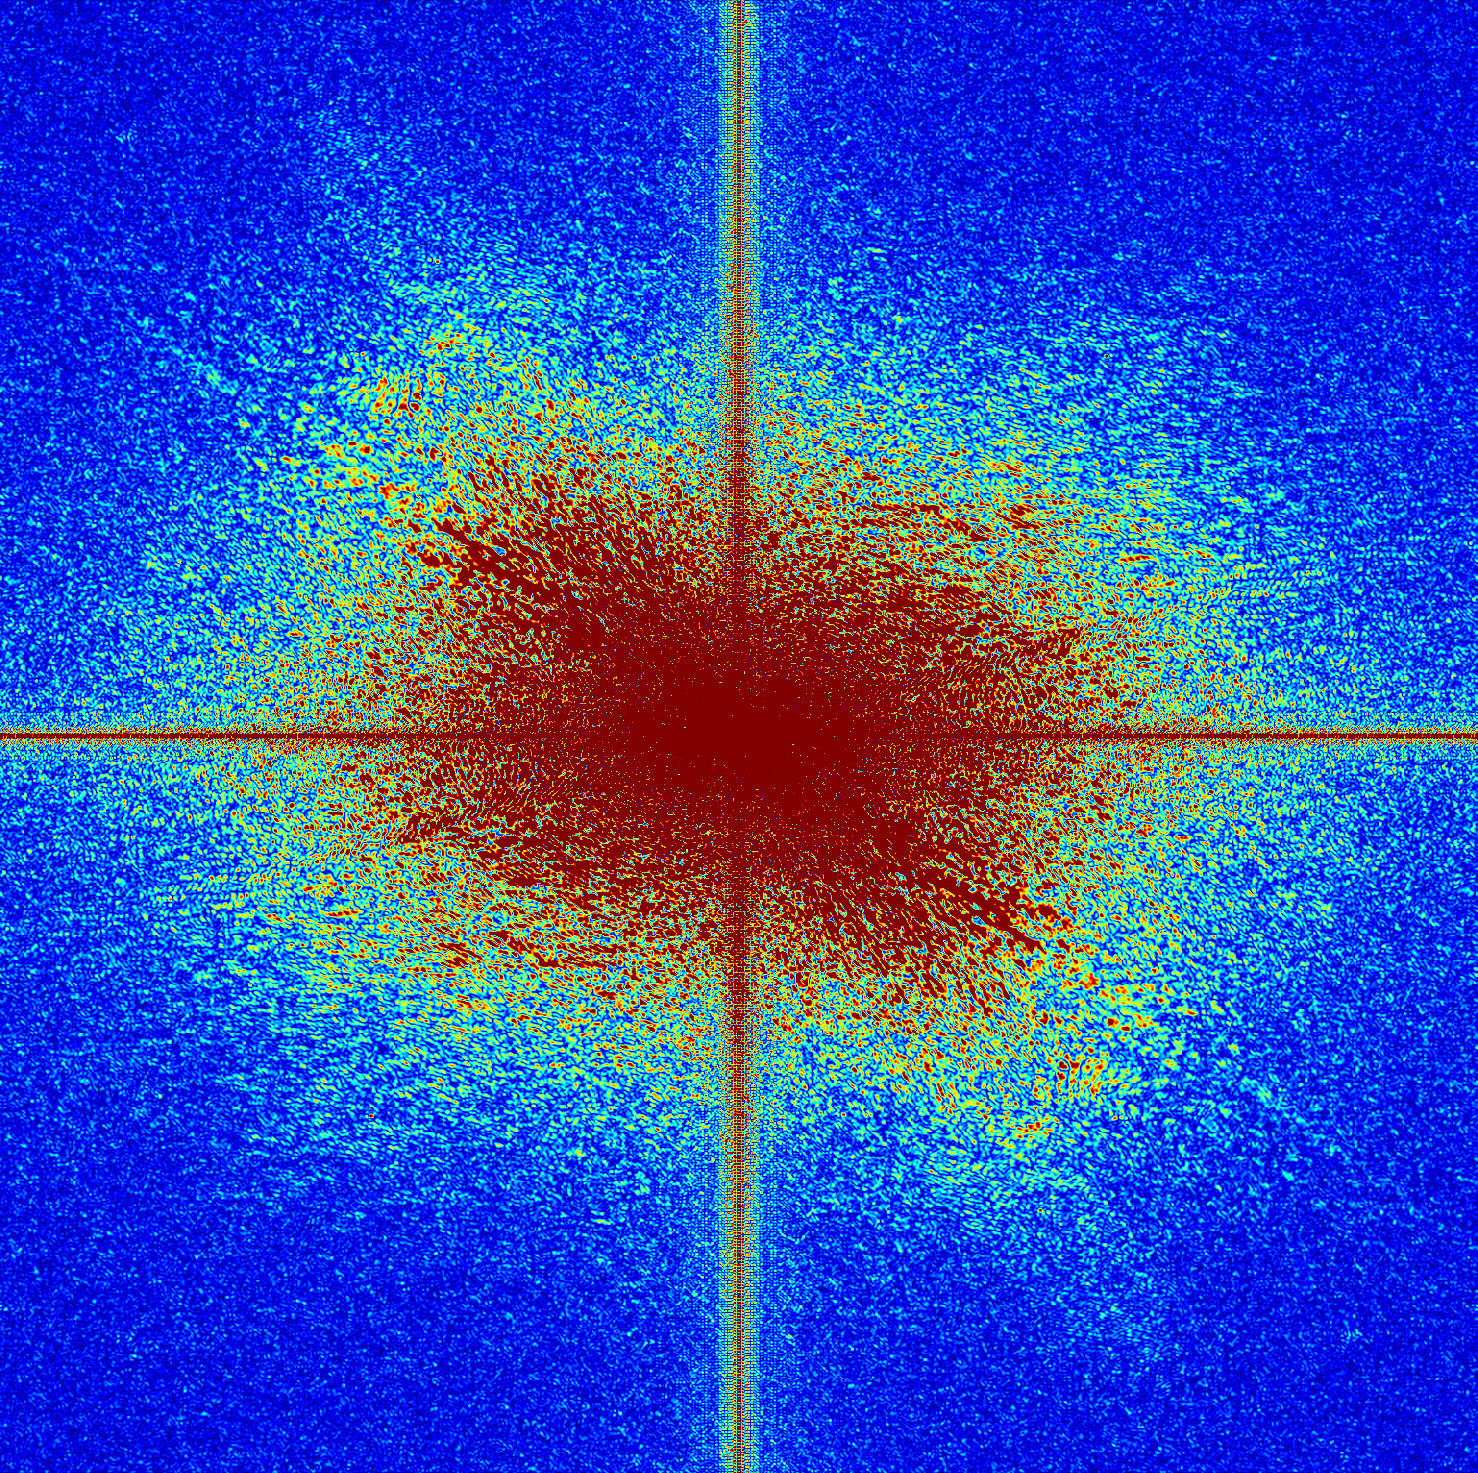
\includegraphics[height=4cm]{images/Lenna_fourier.png}}
            \qquad
            \subfigure[高通滤波后]{\includegraphics[height=4cm]{images/high-pass.png}}
            \qquad
            \subfigure[低通滤波后]{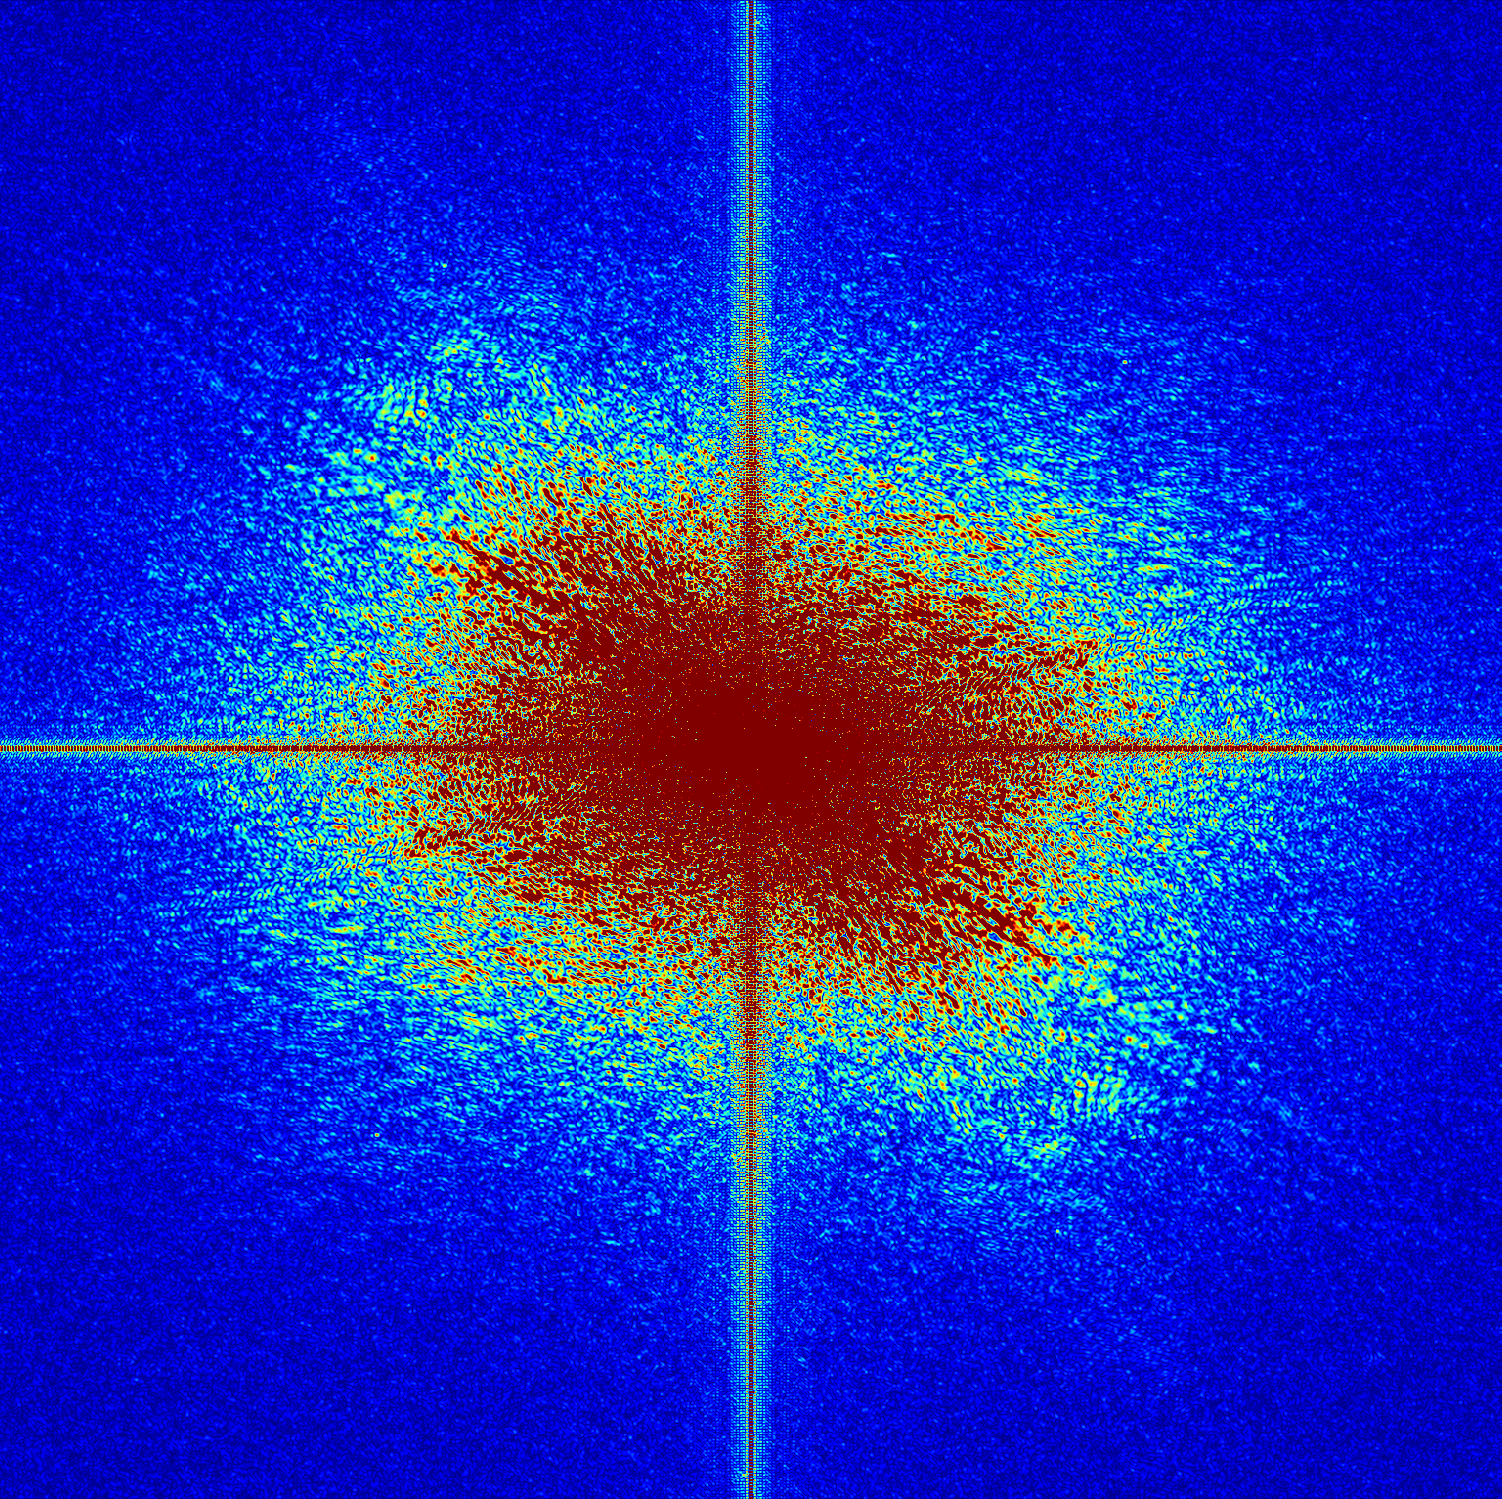
\includegraphics[height=4cm]{images/low-pass.png}}
        \end{figure}
\end{frame}

\begin{frame}
    \frametitle{重建图像对比}
        \begin{figure}
            \subfigure[滤波前]{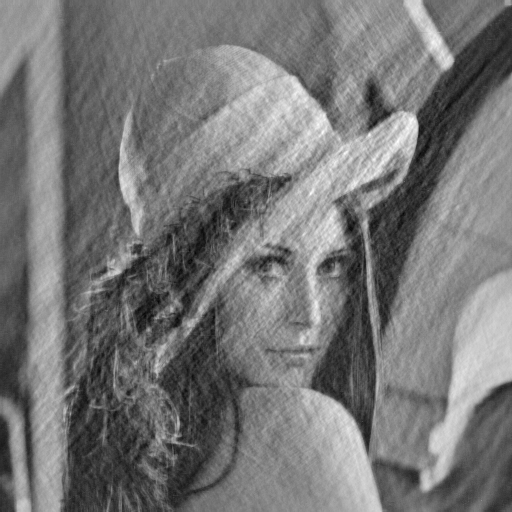
\includegraphics[height=4cm]{images/Lenna_test_1000_180d.png}}
            \qquad
            \subfigure[高通滤波后]{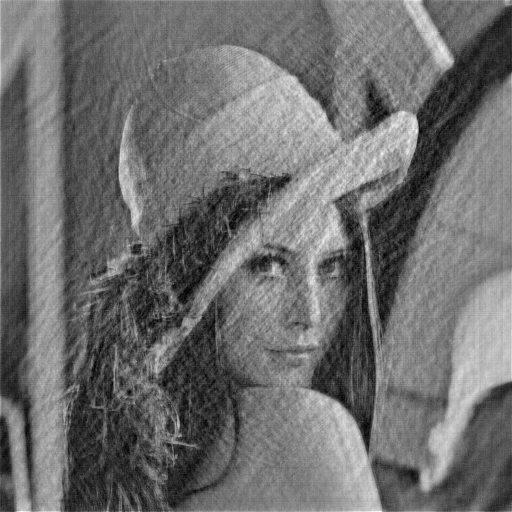
\includegraphics[height=4cm]{images/Lenna_test_RL_0.5.png}}
            \qquad
            \subfigure[低通滤波后]{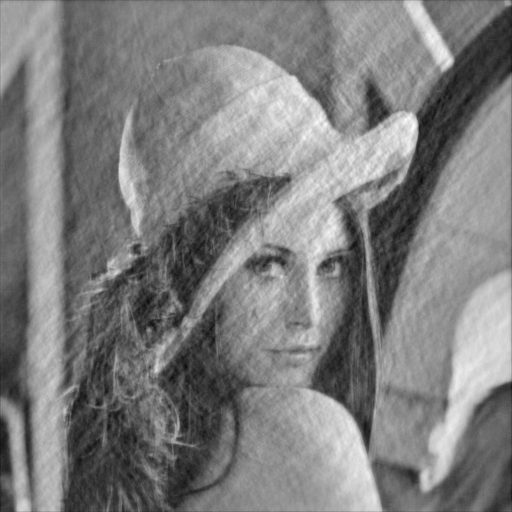
\includegraphics[height=4cm]{images/Lenna_test_RL_0.5_anti.png}}
        \end{figure}
\end{frame}

\begin{frame}
        \begin{figure}
            \subfigure{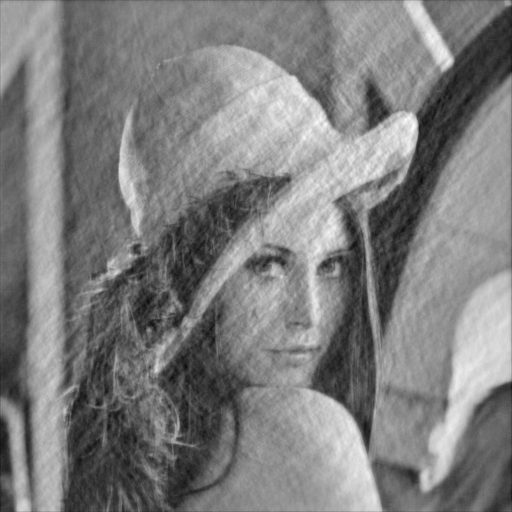
\includegraphics[height=1cm]{images/Lenna_test_RL_0.5_re_0.0.png}}
            \subfigure{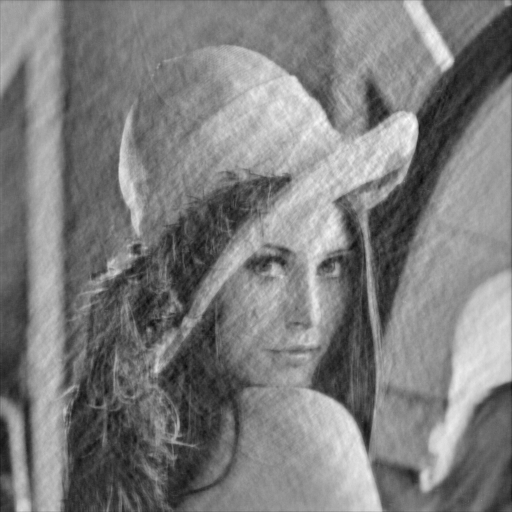
\includegraphics[height=1cm]{images/Lenna_test_RL_0.5_re_0.1.png}}
            \subfigure{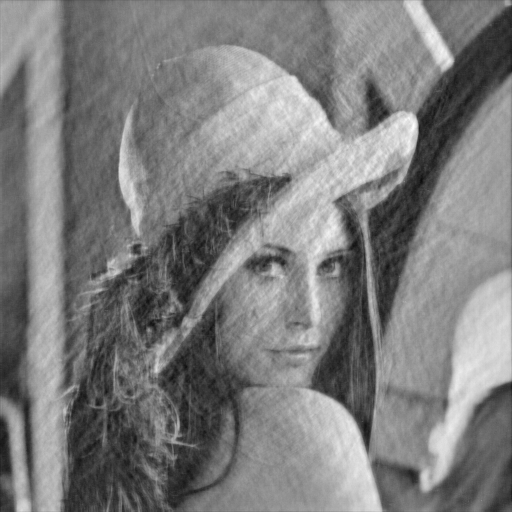
\includegraphics[height=1cm]{images/Lenna_test_RL_0.5_re_0.2.png}}
            \subfigure{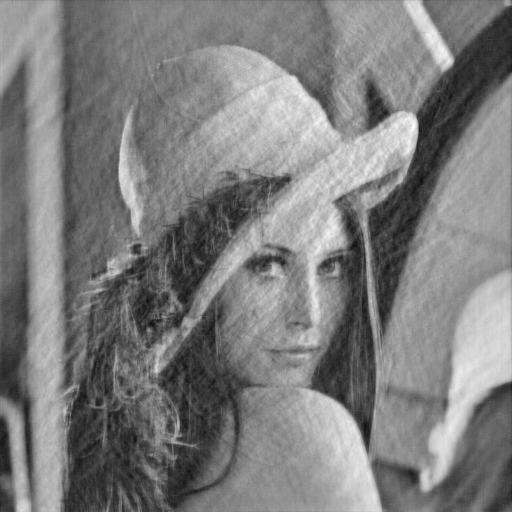
\includegraphics[height=1cm]{images/Lenna_test_RL_0.5_re_0.3.png}}
            \subfigure{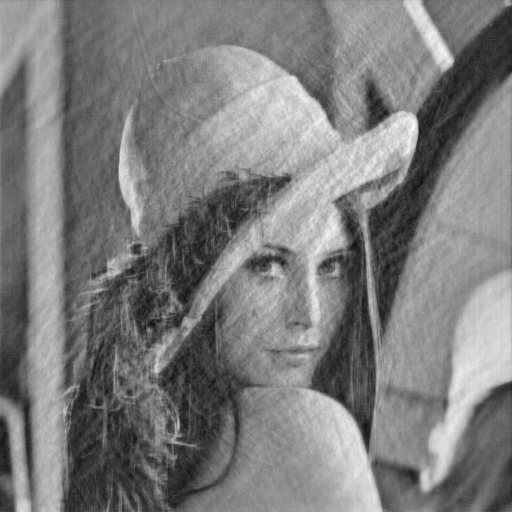
\includegraphics[height=1cm]{images/Lenna_test_RL_0.5_re_0.4.png}}
            \subfigure{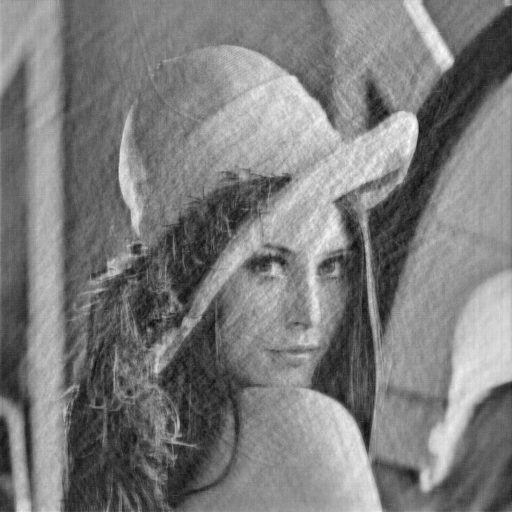
\includegraphics[height=1cm]{images/Lenna_test_RL_0.5_re_0.5.png}}
            \subfigure{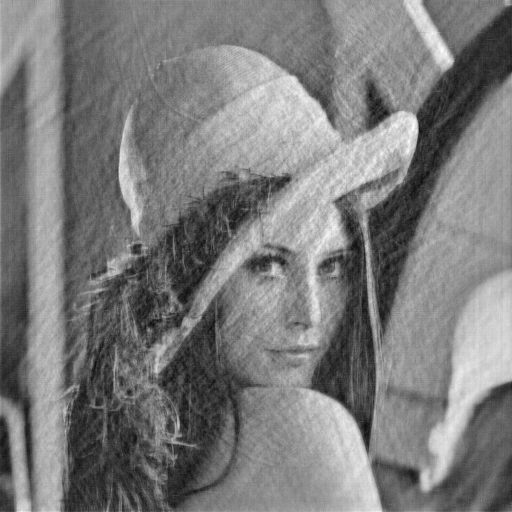
\includegraphics[height=1cm]{images/Lenna_test_RL_0.5_re_0.6.png}}
            \subfigure{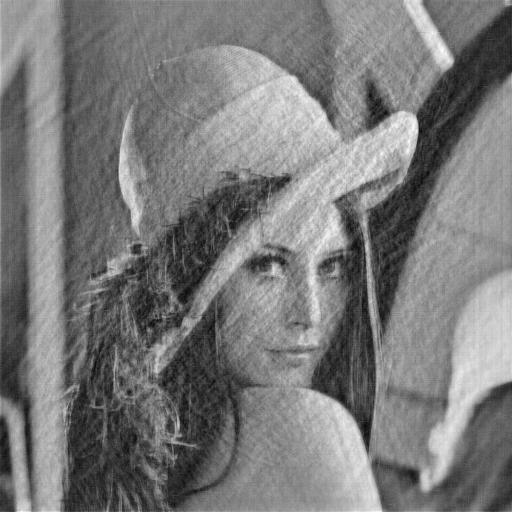
\includegraphics[height=1cm]{images/Lenna_test_RL_0.5_re_0.7.png}}
            \subfigure{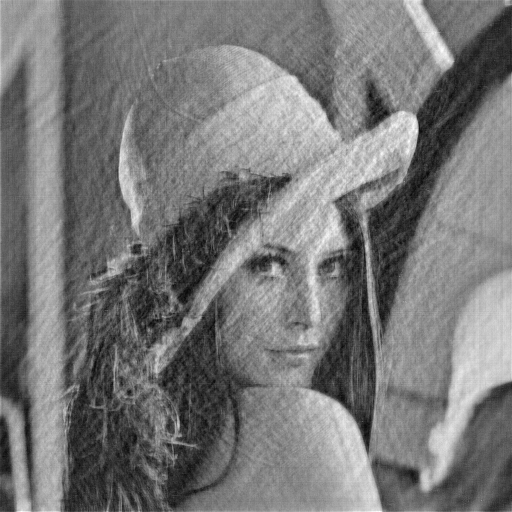
\includegraphics[height=1cm]{images/Lenna_test_RL_0.5_re_0.8.png}}
            \subfigure{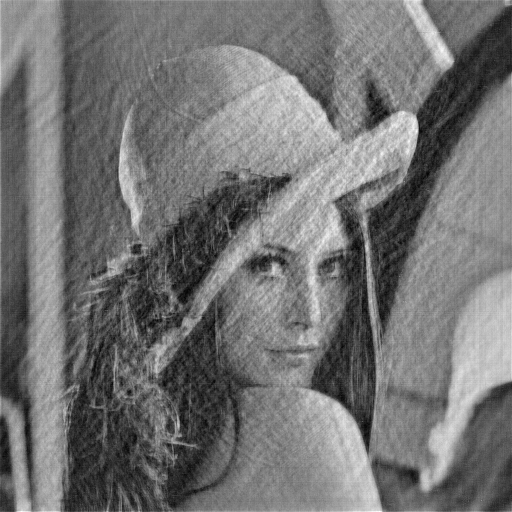
\includegraphics[height=1cm]{images/Lenna_test_RL_0.5_re_0.9.png}}
            \subfigure{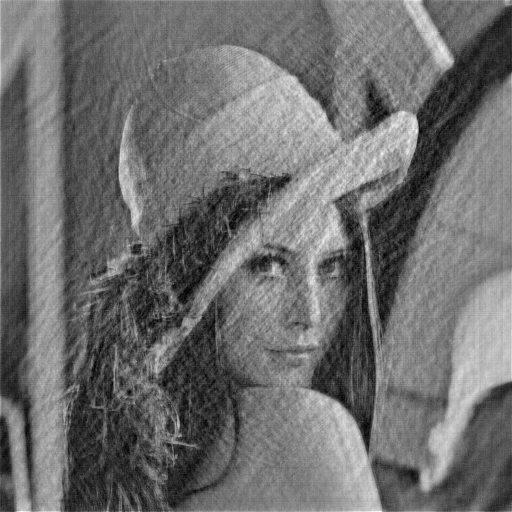
\includegraphics[height=1cm]{images/Lenna_test_RL_0.5_re_1.0.png}}
            \subfigure{\includesvg[height=5cm]{images/rmse.svg}}
        \end{figure}
\end{frame}

\end{document}